\documentclass[../main.tex]{subfiles}
\begin{document}

\thispagestyle{myheadings}

\chapter{Introduction: Background and Literature Review}
\label{sec:introduction}


\section{Optical Imaging of Neural Activity}\label{sec:optical-imaging-of-neural-activity}

Optical techniques for observing neural activity have recently advanced owing to both an evolution of digital imaging technology, and the development of engineered proteins that act as fluorescent indicators of neural activity.
Image sensors, like those found in scientific-CMOS (sCMOS) cameras are larger, faster, and more sensitive than prior scientific grade cameras.
Meanwhile, the latest generation of Genetically Encoded Calcium Indicators (GECIs), collectively called GCaMP6, report fluctuations in neural activation with extremely high fidelity.
This combination of developments enables neuroscientists to open a wider channel to the brain than previously possible using conventional epifluorescence microscopy techniques that enable simultaneous recording from hundreds to thousands of neurons.
Expanding the fraction of the observable neurons in an interconnected network could improve understanding of neural coding and provide insight into mechanistic properties of neural disease.
Additionally, feeding a large set of neural response information to a machine learning algorithm in a neuroprosthetic application may provide improved predictive performance even when the exact mechanism of prediction is difficult to discern.
However, several major challenges currently antagonize the potential benefits of these new technologies:

\begin{enumerate}
	\def\labelenumi{\arabic{enumi}.}
	\itemsep1pt\parskip0pt\parsep0pt
	\item
	      The increased size of raw data from a single imaging session can
	      easily overwhelm the computational resources typically used to process
	      similar but smaller sets of data.
	\item
	      The accumulation of raw data on disk over multiple imaging sessions
	      quickly exceeds the data-storage capacity of most lab-scale servers,
	      forcing researchers to halt data collection to process and delete,
	      potentially creating a ``nightmare scenario''.
	\item
	      The experimental design and data analysis procedures familiar to
	      neuroscientists for network activity data for 5 to 10 cells produce
	      highly biased spurious results in the absence of numerous
	      stimulus-response repetitions, i.e., trials.
	      The number of repeated trials sufficient to produce an accurate description of the neural response to any stimulus is on the order of 2N, where N is the number of neurons being measured.
\end{enumerate}

In the chapters that follow I provide background on the general procedure for offline video processing.
I also discuss some of the issues that limit execution of these procedures on a large dataset, and the variety of approaches that I and others have attempted to address this issue.
I then introduce the streaming approach that is capable of directly processing video during acquisition and extracting signals, thereby saving relevant signals only while also discarding or compressing the raw video.
This approach relies on GPU programming and therefore I also provide background on the application of graphics cards for computationally demanding tasks.
Using a graphics card for programming in the MATLAB environment is also discussed.

Capturing wide-field fluorescence images at high spatial and temporal resolution enables us to measure functional dynamic changes in multiple cells within a large interconnected network.
Extracting a measure for each cell in a way that preserves spatial and temporal continuity with uniform/unbiased sampling of the observed signal is achievable but several factors complicate procedures intended to accomplish this task.
One class of computer-vision procedure commonly applied to this task is image-segmentation (cell-segmentation in histology applications), a procedure that attempts to represent distinct objects in an image by association of each image pixel with one of any number of abstract objects or with the background.
A variety of algorithms exist for efficiently performing this operation on single images.
Most methods can be extended to operate in a 3rd dimension, applied to stacks of image frames to enable tracking cells at multiple depths, or equivalently over time.

However, motion induced by physiologic changes and animal movement necessitates the correct alignment of all frames in the sequence.
Moreover, the massive fluctuations in signal intensity from individual and spatially overlapping cells often breeds unstable solutions for alignment that radically complicate cell identification routines by disrupting temporal continuity.
Implementing a reliable procedure for identifying and tracking the same cells in each frame throughout the sequence thus becomes non-trivial.

\section{Procedures for Calcium Imaging}\label{sec:procedures-for-calcium-imaging}

The general goal of processing image data from functional fluorescence imaging experiments is to restructure raw image data in a way that maps pixels in each image frame to distinct individual cells or subcellular components, called `Regions-Of-Interest' (ROI).
Pixel-intensity values from mapped pixels are often reduced by combination to single dimensional `trace' time-series.
These traces indicate the fluorescence intensity of an individual neuron over time, and the collection approximates the distinct activity of all individual neurons in the microscope's field of view.
However, this task is made difficult by motion of the brain throughout the experiment and by the apparent overlap of cells in the single image plane due to limitations of the camera's 2-dimensional perspective.
These issues can be partially mitigated with a few image pre-processing steps.
Most importantly is the alignment of images to correct for motion.
These options are described in the Methods \& Approaches section below.
Most software packages specifically geared toward functional imaging implement either of two basic classes of pixel-\textgreater{}cell mapping algorithms.
One approach is to use image-segmentation routines for computer vision that seeks to combine adjacent pixels into distinct spatially segregated regions representing objects in the image.

The other common approach is to perform an eigenvalue decomposition on the covariance matrix from a stack of image frames (also called spectral decomposition, or Principal Component Analysis, PCA), resulting in an assembly of basis vectors that define the weighting coefficients for each pixel.
Multiplying the basis-vectors (i.e., ``components'') with all frames produces a one-dimensional trace for each component.
The linear combination is similar to the weighted image-segmentation method in that it assigns fractional coefficients to pixels.
However, the procedure for computing the covariance matrix employed by PCA operates on as many pixels as exist in the image, multiplying each with every other pixel that creates a problem with np2 complexity, where p is the number of pixels in the image.
I mention these issues inherent to PCA not because this project addresses them but because this project was initiated following substantial difficulty attempting to use PCA-based cell sorting methods with large datasets.

\section{Computer Software Environments for Image Processing}\label{sec:computer-software-environments-for-image-processing}

The widespread usage of MATLAB in neuroscience communities lends potential for greater usability and easier adaptation to software developed in this environment.
While software development environments focused on ``ease-of-use'' traditionally presume crippling sacrifices to computational performance, this assumption is now less accurate.

Standard programs include ImageJ, the built-in routines in MATLAB's Image Processing Toolbox, Sci-Kits Image for Python, and a remarkable diversity of miscellaneous applications.
MATLAB is a commercial software development platform that is geared toward fast production and the prototyping of data processing routines in a high-level programming language.
It implements several core libraries (LINPACK, BLAS, etc.)
that make multi-threaded operations on matrix type data highly
efficient.
While MATLAB has traditionally been considered the standard across neuroscience research labs, it is well recognized that its performance was lackluster for ``vectorized'' routines as compared to applications developed using lower-level languages like FORTRAN, C, and C++.
Nevertheless, it remained in common use, and recent releases have added features that can drastically mitigate its poor performance issues, particularly through the development of a ``Just-In-Time'' compiler that automatically optimizes the deployment of computation accelerator resources for standard MATLAB functions.
This feature enables code that performs repeated operations using for-loops or while-loops nearly as fast as equivalent code written in C.
Additionally, code can be compiled into executable format using the Matlab Compiler toolbox, or used to generate equivalent C or C++ code using Matlab Coder.

\section{Computational Resources for Processing Large Data Sets}\label{sec:computational-resources-for-processing-large-data-sets}

Routines for extracting the activity in each cell from a collection of raw imaging data rely on simultaneous access to many pixels separated over space and time (and consequently, are separated on a disk).
For long recording sessions however, the size of the collection of stored image data dramatically grows.
This substantial increase in data size easily exceeds the capacity of system memory in the typical workstation computer available to most researchers.
Thus, performing the necessary processing performance enhancing routines using standard programs is often unfeasible.

Another popular approach to this challenge is the migration of processing routines to a cluster-based system.
In this way, image data can be distributed across many interconnected computer nodes capable of performing all locally restricted image processing procedures in parallel and then passing data to other nodes in the cluster for tasks that rely on comparisons made across time.
Access to clusters capable of performing in this way has been historically restricted to researchers in universities or other large organization, and the diversity of cluster types is sizeable, with clusters often having very particular configuration requirements for efficiently implementing data processing jobs.
These issues pose difficulty to the use and shared development of software libraries for image processing routines, although the growth of ``cloud computing'' services such as Amazon's EC2 and the Google Compute Engine, as well as collaborative computing facilities such as the Massachusetts Green High-Performance Computing Center minimize several of these processing issues.
Additionally, efforts to produce a standardized interface for accessing and distributing data and for managing computing resources across diverse computing environments have seen appreciable success.
Apache's release of the open-source cluster computing framework, Hadoop, and a companion data-processing engine called Spark, have encouraged a massive growth in collaborative development projects, and consequently increased the availability of robust shared libraries for data processing in a variety of applications.
The Spark API can be accessed using the open-source programming Python or other languages including Java, Scala, or R.
The Thunder library, a Spark package released by the Freeman lab and developed in collaboration with a number of other groups at Janelia Farm and elsewhere is specifically geared for image processing of neural imaging data.

Many applications will find that the recent improvements in accessibility and standardization make cluster computing an attractive and worthwhile option for processing large sets of reusable data.
However, this strategy imposes harsh limitations for a neuroscientist engaged in a project that is continuously generating new data, as the time required to transfer entire imaging data sets across the internet may be prohibitive.
Unfortunately, storage capacity on the cloud is also quite finite.
The required capacity to store the accumulated output from continuous high throughput devices such as image sensors.
This rate imbalance is a central motivating issue in this project and is discussed in detail below.

The generation of sCMOS cameras available at the start of this work capture full-frame resolution video at either 30 fps or 100 fps depending on the data interface between camera and computer (USB3.0 or CameraLink).
At 16-bits per pixel and 2048x2048 pixels, the maximum data rate for the USB3.0 camera is 240 MB/s.
Imaging sessions typically last 30-minutes or less.
Pixels are typically binned down 2x2, and frame rate is often reduced to work within the constraints our laboratory workstations impose on processing speed and storage.
However, the effect of doubling resolution on processing time when using the graphics card is virtually negligible.
Identifying ROIs online and extracting the traces of neural activity allows us to discard acquired images and instead, only store the relevant pixels for later analysis.

\subsection{Graphics Processing Units for Video Processing}\label{sec:graphics-processing-units-for-video-processing}

Graphics Processing Units were traditionally developed for the consumer gaming market.
They are optimized for the process that involves translating a continuous stream of information into a two-dimensional image format for transfer to a computer monitor.
In the context of gaming, the stream of information received by a GPU describes the state of objects in a dynamic virtual environment and is typically produced by a video game engine.
These processors are highly optimized for this task.
However, they are equally efficient at performing the same procedure type in reverse, reducing a stream of images to structured streams of information about dynamic objects in the image.
These features render them popular for video processing and computer vision applications.

All GPU architectures consists of a hierarchy of parallel processing elements.
NVIDIA's CUDA architecture refers to the lowest level processing element as ``CUDA Cores'' and the highest level as ``Symmetric Multiprocessors.''
Typically, data is distributed across cores and multiprocessors by specifying a layout in C-code using
different terminology, ``threads'' and ``blocks.'' Blocks are then termed to be organized in a ``grid.''
Adapting traditional image processing or computer vision algorithms to quickly run on a GPU involves efficiently distributing threads and ideally minimizes communication between blocks.

\begin{figure}[b]
\centering
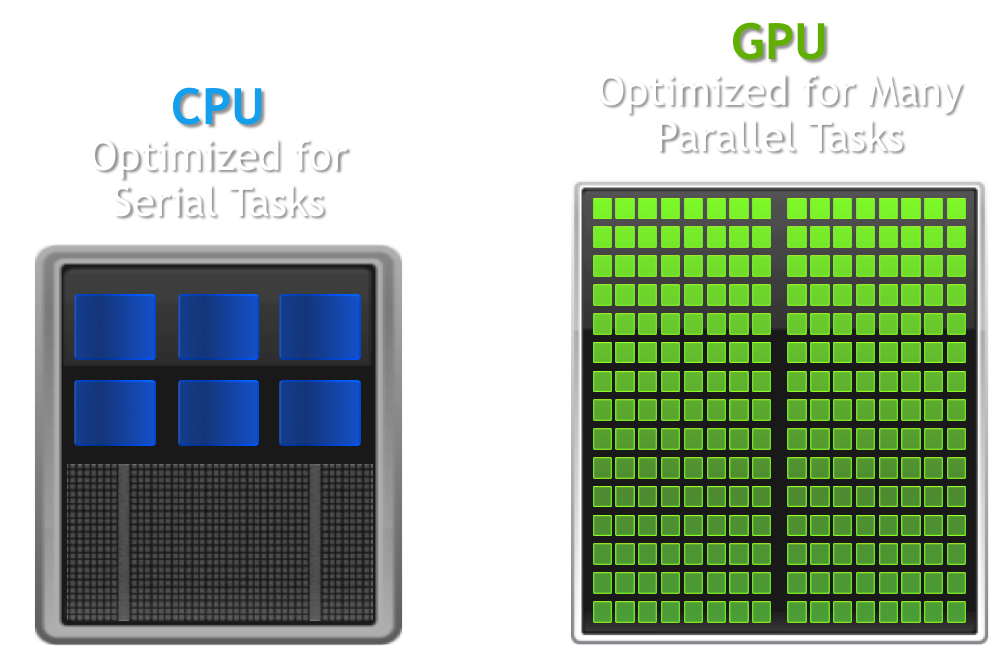
\includegraphics[width=\linewidth]{cpu_vs_gpu.png}
\caption[Comparison of processor architectures]{Comparison of processor architectures: CPU (left) and GPU (right) differ tremendously in the number of ALUs packed on a chip [\url{https://www.datascience.com/blog/cpu-gpu-machine-learning}]}
\label{fig:gpu-comparison}
\end{figure}

MATLAB makes processing data using the GPU seemingly trivial by overloading a large number of built in functions.
Performance varies however.
Writing a kernel-type subfunction is often the fastest way to implement a routine written as if it operates on single (scalar) element only that can be called on all pixels at once or employs all pixel-subscripts used by the function to retrieve the pixel value at a given subscript.
The kernel-type function is compiled into a CUDA kernel the first time it's called, then repeated calls directly contact the kernel with minimal overhead.
Calls typically use the arrayfun() function.

Data transfers between system memory and graphics memory is often a major bottle-neck.
Therefore, this operation is best performed only once.
However, once data is available to the GPU, many complex operations can be performed to extract information from the image without exceeding the processing-time limit imposed by the frame-rate of the camera sending the images.

In total, this project employs advances in both software and hardware that facilitate rapid accurate image analysis of living organisms with the ultimate goals of simplifying the acquisition and analysis of neural activity indicators in both normal and pathological states.

\clearpage

\end{document}

\cleardoublepage{}
